
%%%%%%%%%%%%%%%%%%%%%%%%%%%%%%%%%%%%%%%%%%%%%%%%%%%%%%%%%%%%%%%%%
%                                                               %
% Chapter: asymmetries Wed Sep 25 16:01:23 EDT 2013
%                                                               %
%%%%%%%%%%%%%%%%%%%%%%%%%%%%%%%%%%%%%%%%%%%%%%%%%%%%%%%%%%%%%%%%%

\chapter{Calculation of single-$\mu$ asymmetries}
\label{ch:asymmetries}

\section{Crossing information}
Once the signal and background ratios are defined, one can continue on towards the asymmetry calculation. 
At this point, the run13 spin database contains already the final spin patterns and crossing shifts, 
so the official database information are used for the asymmetries evaluation. However, as a cross check, the crossing distribution after taking into 
account the shift from the spin database is plotted in order to make sure, the correct shift is applied. Fig.~\ref{fig:crossingdist} 
displays this crossing information for all muon candidates with transverse momenta above 16\,GeV/$c$ and otherwise minimal requirements.
 The distributions does not show any substantial entries in the empty  crossings 28/29, 69/70 at the beginning of run13.

\begin{figure}[ht]
\begin{center}
\includegraphics[width=\textwidth]{../asymmetries/figs/run13/crosscheck13.png}
\caption{Crossing distribution for muon candidates with transverse momenta above 16\,GeV/$c$ for the North (bottom panel) and South (top panel) arms and for positive (right) and negative (left) tracks as a function of frunnumber. \label{fig:crossingdist}}
\end{center}
\end{figure}

\section{Asymmetry calculation}
After confirming the correct crossing and hence spin pattern information the actual raw asymmetries can be calculated similar to 
the run11 and run12 preliminary results \cite{cite:run11W,cite:run12W} by separating all muon candidates of a certain preselection range into the 4 different spin states 
for each arm and charge separately. 
For the asymmetry calculation the yields were summed up over all runs and fills as the statistics are too limited to calculate fill-by-fill asymmetries.
For a particular preselection level, and minimum transverse momentum cut, the yields are then calculated for the 4 separate spin states as shown for 
example in Fig.~\ref{fig:asyrawlowf}.
\begin{figure}[ht]
\begin{center}
\includegraphics[width=\textwidth]{{../asymmetries/figs/run13/asy13_16_60_fcut-0.00_0.04_wness_dw0}.png}
\caption{Raw spin separated yields taking also the lowest (background-dominated) likelihood ratios $f_{cut} >0.0$ into account \label{fig:asyrawlowf}.}
\end{center}
\end{figure}

They are fit by the following function for each arm and charge:
\begin{equation}
N^{\alpha,\beta} = \sigma_0 + \alpha \sigma_{L}^{Blue} + \beta \sigma_{L}^{Yellow} + \alpha \beta \sigma_{LL}\quad,
\end{equation}
\noindent where $\alpha$ ($\beta$) are the two spin states ($\pm 1$) for the blue (yellow) beam respectively. The corresponding asymmetries are then obtained by 
normalizing the spin dependent terms by the unpolarized term and the corresponding average beam polarization(s):
\begin{eqnarray}
A_{L}^{Blue} &=& \frac{\sigma_{L}^{Blue}}{<P^{Blue}>\sigma_0} \\
A_{L}^{Yellow} &=& \frac{\sigma_{L}^{Yellow}}{<P^{Yellow}>\sigma_0} \\
A_{LL} &=& \frac{\sigma_{LL}}{<P^{Blue}><P^{Yellow}>\sigma_0}\quad
\end{eqnarray}
The asymmetry values before normalizing with the average polarizations are commonly referred to as $\epsilon_L$ and $\epsilon_{LL}$. 

As seen in Fig.~\ref{fig:asyrawlowf} the background dominated events all give raw asymmetries consistent with 
zero and at high precision compared to the signal enhanced sample. This is consistent with the expectation of no parity 
violating asymmetries and therefore the signal asymmetries needs to be corrected only for dilution, but no additional asymmetry. 
The results of the naive single spin asymmetries (ie $\frac{N^+ -N^-}{N^++N^-}$ for one beam while disregarding the other beam's helicities)
 are also shown and are in agreement with the fit results.  

The corresponding yields and raw asymmetries for the signal region are displayed in Fig.~\ref{fig:asyrawhighf}. 
One immediately sees, that the statistics are significantly lower and that the yields are not as evenly distributed between the 
different spin states indicating nonzero asymmetries. 

\begin{figure}[ht]
\begin{center}
\includegraphics[width=\textwidth]{{../asymmetries/figs/run13/asy13_16_60_fcut0.92_wness_dw0}.png}
\caption{Raw spin separated yields taking the tightest (signal-enhanced) selection criterion $f_{cut} > 0.92$ \label{fig:asyrawhighf}}
\end{center}
\end{figure}


As a summary of the raw asymmetries calculations all preselection regions are displayed in Fig.~\ref{fig:asyvsfcut}. The very small asymmetries at very low W likelihoods stick out as well as the very high likelihood region which is the only region with nonzero asymmetries at the one sigma level.  
\begin{figure}[ht]
\begin{center}
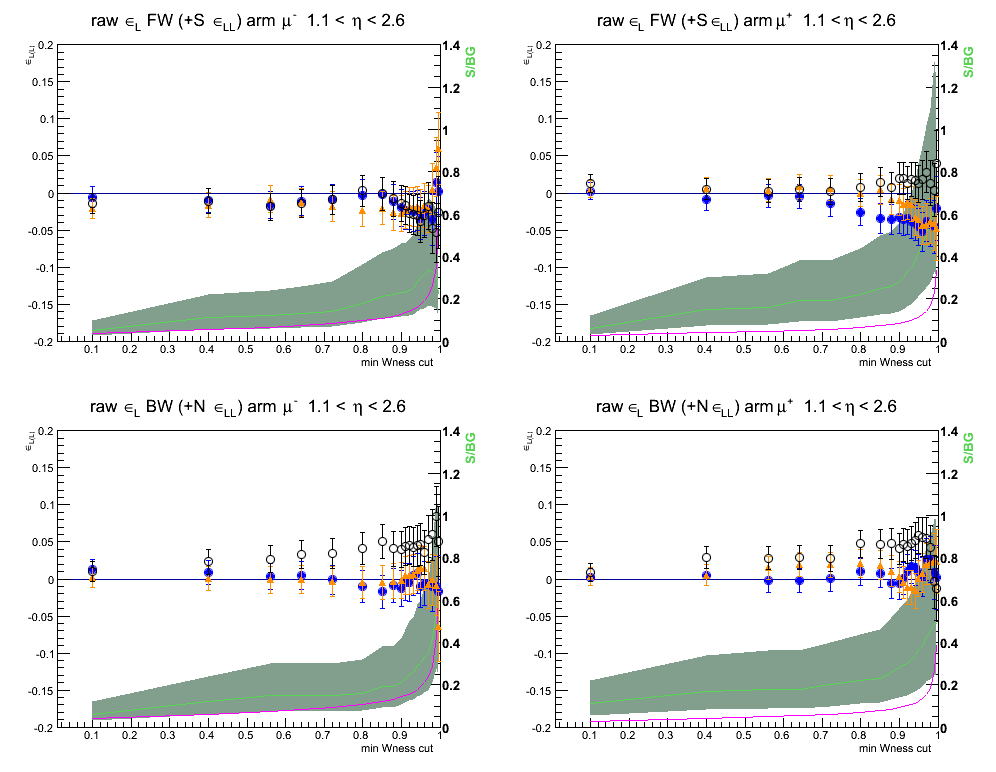
\includegraphics[width=\textwidth]{{../asymmetries/figs/run13/asyvsfcut13_wness_eta3_16_60_dw0}.png}
\caption{Raw asymmetries $\epsilon_{L}$ for the Blue (blue symbols) and Yellow (orange symbols) beams and $\epsilon_{LL}$ (black symbols) for both arms and charges as a function of the preselection range. The combination of all rapidities in one bin after selecting the central dw23 region is displayed. In addition the extracted signal to background ratios are displayed using the right-hand axis values. The green line displays the data-based extraction method while the magenta line represents the MC signal based extraction.\label{fig:asyvsfcut}}
\end{center}
\end{figure}




\subsection{Asymmetry dependence on RPC combinations in preselections }
% Using the different RPC1 and 3 combinations for the preslection partially overlapping final data sets with minimum
%likelihood ratios of 0.92 can be obtained. We are studying how the asymmetries vary varying the combinations of detectors
%used in the wness.{\color{red} The results of this test will be updated soon in this
%note.}
The corresponding asymmetries $\epsilon_L$, already ordered forward or backward pointing, are displayed in Fig.~\ref{fig:asy_wnessdiff} the three rapidity bins as well as combined. 
{\color{red} need to update plot}

\begin{figure}[ht]
\begin{center}
\includegraphics[width=\textwidth]{../asymmetries/figs/run13/asy_wnessdiffs13.pdf}
\caption{Raw asymmetries $\epsilon_{L}$ for the Blue (blue symbols) and Yellow (orange symbols) beams in the forward (top) and backwards (bottom) direction relative to the polarized beam for the preselection range above 0.92. The different points show the different rapidity bins (open symbols) and their average (full symbols). \label{fig:asy_wnessdiff}}
\end{center}
\end{figure}



To obtain actual asymmetries the raw asymmetries need to be normalized by the average polarizations which were taken as 
$54 \pm 0.42 \%$ for the Blue beam and $55 \pm 0.40 \%$ for the Yellow beam according to the offline values~\cite{cite:cnipols}. 
Currently the overall averages are being used rather than fill weighted averages as the differences are not expected to be substantial 
at this point. 


The individual and combined asymmetries for three different $\eta$ bins, $1.10 < \eta < 1.40$, $1.40 < \eta < 1.80$ and
 $1.80 < \eta < 2.60$, are summarized in Table \ref{Tab:Dat:finalasy} before and after background correction and combination. % which are not yet background corrected.
%\begin{table}
%\begin{center}
%\caption{Summary of beam separated single and double spin asymmetries together with their uncertainties using the likelihood level of $wness > 0.92$ and transverse momenta above 16\,GeV/$c$ before correcting for background.\label{tab:finalasy1}{\color{red} need to update}}
%\begin{tabular}{|c|rr|rr|}
%\multicolumn{5}{c}{$A_L$} \\ \hline
%Chrg & $\eta_B$ & $A_{B}$& $\eta_Y$& $A_{Y}$ \\ \hline
%$\mu^{+}$ &  $-1.30$ & $0.011\pm 0.052$  &  $1.31$ & $0.016\pm 0.049$ \\%south
%  &  $-1.59$ & $0.019\pm 0.027$ & $-1.59$ &  $-0.000\pm 0.026$\\
%  &  $-1.99$ & $0.042\pm 0.035$ &$-2.03$ &  $0.020 \pm0.030$ \\
%$\mu^{+}$ &  $-1.31$ & $-0.139\pm 0.048$ &  $1.30$& $-0.011\pm 0.052$  \\
%& $-1.59$ & $0.0055\pm 0.026$  &  $1.59$&  $-0.027\pm 0.027$ \\
%&$-2.03$ & $-0.0036\pm 0.030$  &  $1.99$&  $0.032\pm 0.035$   \\
%$\mu^{-}$ &$-1.30$ & $0.032\pm 0.063$ &$1.31$&  $0.088\pm 0.063$\\
%&$-1.61$ & $0.0089\pm 0.032$ & $1.61$ & $0.021\pm 0.030$ \\
%&$-2.01$ & $-0.0053\pm 0.036$ & $2.04$ & $-0.035\pm 0.033$ \\
%$\mu^{-}$ &$-1.31$ & $-0.016\pm 0.063$ &$1.30$ &  $0.089\pm 0.063$  \\
%& $-1.61$ & $0.0064\pm 0.030$ &$1.61$ & -$0.013\pm 0.032$\\
%& $-2.04$ & $0.024\pm 0.033$ &$2.01$ & $0.0027\pm 0.036$\\
%\hline
%\multicolumn{5}{c}{$A_{LL}$} \\ \hline
%Chrg & $\eta_S$ & $A_{LL}$& $\eta_N$ & $A_{LL}$\\ \hline
%$\mu^{+}$ &  $1.30$  & $0.054\pm 0.052$  & $1.31$ & $-0.012\pm 0.049$\\
%&  $1.59$ &   $0.019\pm 0.027$ & $1.59$ &$0.066\pm 0.026$  \\
%& $1.99$& $ -0.012\pm2 0.035$ & $2.03$& $ 0.0036\pm 0.030$\\
%$\mu^{-}$ & $1.30$& $-0.153\pm 0.063$ & $1.31$ & $0.016\pm 0.063$\\
%&$1.61$& $-0.059\pm 0.032$& $1.61$ &$0.037\pm 0.030$\\
%&$2.03$ & $0.064\pm 0.036$ & $2.04$ &$0.076\pm 0.033$\\
%\hline
%\end{tabular}
%\end{center}
%\end{table}


\subsection{Cross check}
The raw asymmetries have been calculated currently by Francesca and Ralf based on a Ralf preselection TTree and using independent analysis codes which access the spin database and calculate the corresponding asymmetries. 
The selected event yields
as well as the simple and fitted single and double spin asymmetries are in perfect agreement within the leading 3 digits of the calculations,
which indicates a correct treatment of the asymmetries. Assuming no sign change between the database spin orientations from the CNI 
polarimeter position and at PHENIX ( ie up transverse polarization at the CNI becomes a positive helicity at PHENIX) the overall sign of the 
asymmetries was determined. 
Also the mapping of positive, negative charge, north, south and the corresponding forward/backward orientation for the corresponding 
polarized beams were confirmed.   

\subsection{Bunch Shuffling}\label{sec:bunch_shuf}
A further test that can be done to check for any systematic flaws in the asymmetry calculation method and to confirm accurate asymmetry
uncertainties is bunch shuffling. Bunch shuffling is an exercise consisting of many iterations of randomizing the spin pattern associated
with each event. After each randomization, the resulting asymmetries are calculated and the distribution of asymmetries over all iterations
is studied. The mean of this distribution is expected to be consistent with zero and it's width represents the uncertainty associated with
the asymmetry calculation, so an RMS matching the asymmetry uncertainty offers confirmation of the uncertainty calculation.

The bunch shuffling for this analysis employs two randomizing schemes separately to serve as a cross check. The first is a fill-by-fill
bunch shuffling: for each fill, the spin configuration from each valid crossing of the 120 crossings are swapped randomly with configurations
from other valid crossings. This shuffled mapping is then used when retrieving spin configurations for each event in the fill. Resulting
distributions of asymmetries from this randomization scheme are shown in figures \ref{fig:bnshf_shuf_alb}, \ref{fig:bnshf_shuf_aly}, 
              and \ref{fig:bnshf_shuf_all}. The second randomization scheme is a
pure randomization, where each event is randomly assigned one of the four possible spin configurations. Results from this scheme are shown in
figure \ref{fig:bnshf_rand_alb}, \ref{fig:bnshf_rand_aly} and \ref{fig:bnshf_rand_all}.

\begin{figure}\label{fig:bnshf_shuf_alb}
\includegraphics[width=\textwidth]{../asymmetries/figs/run13/bunshf_alb_shuff.png}
\caption{Distribution of scaled $A_{L}$ for the blue beam from fill-by-fill shuffling bunch shuffling technique. Distribution generated from 100000
randomization iterations. The Asymmetry value is scaled by a factor of the uncertainty of the analysis asymmetry calculation. The result is that
an RMS of 1 for the scaled asymmetry distribution corresponds to an RMS equal to the uncertainty if the unscaled distribution was plotted. Shown
for all arm and charge combinations.}
\end{figure}

\begin{figure}\label{fig:bnshf_shuf_aly}
\includegraphics[width=\textwidth]{../asymmetries/figs/run13/bunshf_aly_shuff.png}
\caption{Distribution of scaled $A_{L}$ for the yellow beam from fill-by-fill shuffling bunch shuffling technique. Distribution generated from 100000
randomization iterations. The Asymmetry value is scaled by a factor of the uncertainty of the analysis asymmetry calculation. The result is that
an RMS of 1 for the scaled asymmetry distribution corresponds to an RMS equal to the uncertainty if the unscaled distribution was plotted. Shown
for all arm and charge combinations.}
\end{figure}

\begin{figure}\label{fig:bnshf_shuf_all}
\includegraphics[width=\textwidth]{../asymmetries/figs/run13/bunshf_all_shuff.png}
\caption{Distribution of scaled $A_{LL}$ from fill-by-fill shuffling bunch shuffling technique. Distribution generated from 100000
randomization iterations. The Asymmetry value is scaled by a factor of the uncertainty of the analysis asymmetry calculation. The result is that
an RMS of 1 for the scaled asymmetry distribution corresponds to an RMS equal to the uncertainty if the unscaled distribution was plotted. Shown
for all arm and charge combinations.}
\end{figure}

\begin{figure}\label{fig:bnshf_rand_alb}
\includegraphics[width=\textwidth]{../asymmetries/figs/run13/bunshf_alb_rand.png}
\caption{Distribution of scaled $A_{L}$ for the blue beam from pure randomization bunch shuffling technique. Distribution generated from 100000
randomization iterations. The Asymmetry value is scaled by a factor of the uncertainty of the analysis asymmetry calculation. The result is that
an RMS of 1 for the scaled asymmetry distribution corresponds to an RMS equal to the uncertainty if the unscaled distribution was plotted. Shown
for all arm and charge combinations.}
\end{figure}

\begin{figure}\label{fig:bnshf_rand_aly}
\includegraphics[width=\textwidth]{../asymmetries/figs/run13/bunshf_aly_rand.png}
\caption{Distribution of scaled $A_{L}$ for the yellow beam from pure randomization bunch shuffling technique. Distribution generated from 100000
randomization iterations. The Asymmetry value is scaled by a factor of the uncertainty of the analysis asymmetry calculation. The result is that
an RMS of 1 for the scaled asymmetry distribution corresponds to an RMS equal to the uncertainty if the unscaled distribution was plotted. Shown
for all arm and charge combinations.}
\end{figure}

\begin{figure}\label{fig:bnshf_rand_all}
\includegraphics[width=\textwidth]{../asymmetries/figs/run13/bunshf_all_rand.png}
\caption{Distribution of scaled $A_{LL}$ from the pure randomization bunch shuffling technique. Distribution generated from 100000
randomization iterations. The Asymmetry value is scaled by a factor of the uncertainty of the analysis asymmetry calculation. The result is that
an RMS of 1 for the scaled asymmetry distribution corresponds to an RMS equal to the uncertainty if the unscaled distribution was plotted. Shown
for all arm and charge combinations.}
\end{figure}

As seen in plots from both techniques, the RMS of a Gaussian fit of the shuffled asymmetry distributions is consistent with the uncertainty 
values extracted from the asymmetry calculations. This adds confidence to the uncertainties. Also, the distribution means are predominantly 
consistent with zero within uncertainties. While this consistency does not explicitly confirm accuracy of our asymmetry calculations, it 
is a sanity check that excludes the presence of possible systematic flaws in our analysis techniques.


\subsection{Background correction}\label{sec:bcg_correc}
Before finalizing the asymmetries one needs to correct for the amount of background events still contained in the final event selection. 
Unlike in other asymmetry extractions, where an obvious invariant mass or Jacobian peaks allows a simple data driven evaluation of the 
background fractions as well as their asymmetries, the forward W decay muon distributions do not have this luxury. However, using the 
shape of the signal distributions from MC it is possible to obtain the signal to background ratio in a nearly entirely data-driven method 
as described in Chapter~\ref{ch:dataanalysis}. %was \ref{chapter:snextraction}. 
As the W related asymmetries are the only parity violating asymmetries the background asymmetries which are dominated by other decay 
muons as well as falsely reconstructed pions and kaons do not contain any nonzero asymmetry. This has been confirmed in the previous 
section where both the asymmetries at the lowest cut levels as well as those at low transverse momenta were consistent with zero. 
Consequently only the dilution of the obtained asymmetries by the background needs to be corrected which is:
\begin{equation}
A_{BGCorr} = A_{meas} (1 + BG / S )\quad,
\end{equation}
\noindent where $A_{meas}$ is the measured asymmetry, S/BG is the signal-to-background ratio and $A_{BGCorr}$ is the background 
corrected asymmetry. The same scale factor is also applied to the statistical uncertainties.


\subsection{Combination of results}
 Finally the single spin asymmetries for both beams can be combined to obtain the very final results. This is performed by 
averaging both results taking into account the final statistical and systematic uncertainties.
All raw and  background corrected single spin asymmetries for the individual beams as well as combined are summarized in Table
~\ref{Tab:Dat:finalasywholeeta} for the whole eta range and in~\ref{Tab:Dat:finalasy} for the separated 3 eta bins
together with the systematic uncertainties. Currently a factor of 2 is assigned on the signal to background ratio.



\begin{table}
\begin{center}
\caption{BG corrected single spin asymmetries $A_L$ for the whole eta range as a function of rapidity with minimum transverse momentum of 
16\,GeV/$c$ with and without combining the two beams and using a minimum $W$ likelihood level of $f_{cut} > 0.92$. 
The signal to background values were extracted from the unbinned maximum likelihood fit. A factor two uncertainty on the 
S/BG value is given as a systematic error band.\label{Tab:Dat:finalasywholeeta}}
\begin{tabular}{|c c c |c c | c|c| c|}
%\begin{tabular}{|c|ccc|cc|}
\hline 
Arm & charge & beam & etabin &  eta & S$/$BG & raw $A_L$ & corrected  $A_L$ \\ \hline   
  N &     +  &   B  &  whole range  &  1.70 & 0.30 & $-0.034\pm  0.022$ & $  -0.272\pm  0.18 ^{0.10} _{0.21} $\\
  S &     +  &   Y  & whole range &  1.67 & 0.33 & $-0.013\pm  0.022$ & $ -0.096 \pm 0.16 6{0.04} _{0.07}$ \\ 
 FW &     +  & comb & whole range &  1.68 & &&$  -0.180 \pm 0.12 6{ -0.23} _{0.17} $\\ \hline 
  S &     +  &   B  & whole range  & -1.67 & 0.33 & $ 0.010\pm  0.022$ & $   0.075\pm  0.17 ^{0.03} _{0.06} $\\
  N &     +  &   Y  & whole range  & -1.70 & 0.30 & $-0.012\pm  0.022$ & $ -0.092 \pm 0.18 6{0.04} _{0.07}$ \\ 
 BW &     +  & comb & whole range  & -1.68 & &&$  -0.006 \pm 0.12 6{ -0.03} _{0.07} $\\ \hline 
  N &     -  &   B  & whole range  &  1.74 & 0.25 & $-0.024\pm  0.026$ & $  -0.223\pm  0.24 ^{0.09} _{0.18} $\\
  S &     -  &   Y  & whole range  &  1.73 & 0.24 & $-0.018\pm  0.026$ & $ -0.166 \pm 0.24 6{0.07} _{0.13}$ \\ 
 FW &     -  & comb & whole range  &  1.74 & &&$  -0.195 \pm 0.17 6{ -0.25} _{0.17} $\\ \hline 
  S &     -  &   B  & whole range  & -1.73 & 0.24 & $-0.005\pm  0.026$ & $  -0.044\pm  0.25 ^{0.02} _{0.04} $\\
  N &     -  &   Y  & whole range  & -1.74 & 0.25 & $ 0.005\pm  0.026$ & $  0.049 \pm 0.23 6{0.02} _{0.04}$ \\ 
 BW &     -  & comb & whole range  & -1.74 & &&$   0.003 \pm 0.17 6{ -0.01} _{0.04} $\\ \hline 
%channel & $\eta$ & RB $\sigma_{W+Z} \times BR$ [pb] & S/BG & raw $A_L$ & corrected $A_L$ \\ \hline 
%N $\mu^{+} B $ & 1.31 & 131  & 0.38 & $-0.14$ & $ -0.93\pm0.33^{0.34}_{0.68}  $ \\ 
%S $\mu^{+} Y $ & 1.30 & 131  & 0.52 &$-0.01$ & $ -0.07\pm0.32^{0.02}_{0.05}  $ \\ 
%N $\mu^{+} B $ & 1.59 & 131  & 0.38 & $0.01$ & $ 0.04\pm0.18^{0.01}_{0.03}  $ \\ 
%S $\mu^{+} Y $ & 1.59 & 131  & 0.52 &$-0.03$ & $ -0.17\pm0.17^{0.06}_{0.12}  $ \\ 
%N $\mu^{+} B $ & 2.03 & 131  & 0.38 & $-0.00$ & $ -0.02\pm0.20^{0.01}_{0.02}  $ \\ 
%S $\mu^{+} Y $ & 1.99 & 131  & 0.52 &$0.03$ & $ 0.20\pm0.22^{0.07}_{0.14}  $ \\ 
%
%S $\mu^{+} B $ & -1.30 & 131  & 0.41 & $0.01$ & $ 0.07\pm0.33^{0.02}_{0.05}  $ \\ 
%N $\mu^{+} Y $ & -1.31 & 131  & 0.38 &$0.02$ & $ 0.11\pm0.32^{0.04}_{0.08}  $ \\ 
%S $\mu^{+} B $ & -1.59 & 131  & 0.41 & $0.02$ & $ 0.12\pm0.17^{0.04}_{0.09}  $ \\ 
%N $\mu^{+} Y $ & -1.59 & 131  & 0.38 &$-0.00$ & $ -0.00\pm0.17^{0.00}_{0.00}  $ \\ 
%S $\mu^{+} B $ & -1.99 & 131  & 0.41 & $0.04$ & $ 0.27\pm0.22^{0.10}_{0.19}  $ \\ 
%N $\mu^{+} Y $ & -2.03 & 131  & 0.38 &$0.02$ & $ 0.13\pm0.20^{0.05}_{0.09}  $ \\ 
%
%N $\mu^{-} B $ & 1.31 & 41  & 0.52 & $-0.02$ & $ -0.09\pm0.34^{0.03}_{0.06}  $ \\ 
%S $\mu^{-} Y $ & 1.30 & 41  & 0.19 &$0.09$ & $ 1.01\pm0.72^{0.42}_{0.85}  $ \\ 
%N $\mu^{-} B $ & 1.61 & 41  & 0.52 & $0.01$ & $ 0.03\pm0.16^{0.01}_{0.02}  $ \\ 
%S $\mu^{-} Y $ & 1.61 & 41  & 0.19 &$-0.01$ & $ -0.15\pm0.36^{0.06}_{0.12}  $ \\ 
%N $\mu^{-} B $ & 2.04 & 41  & 0.52 & $0.02$ & $ 0.13\pm0.18^{0.04}_{0.09}  $ \\ 
%S $\mu^{-} Y $ & 2.01 & 41  & 0.19 &$0.00$ & $ 0.03\pm0.41^{0.01}_{0.03}  $ \\ %
%
%S $\mu^{-} B $ & -1.30 & 41  & 0.19 & $0.03$ & $ 0.37\pm0.74^{0.16}_{0.31}  $ \\ 
%N $\mu^{-} Y $ & -1.31 & 41  & 0.41 &$0.09$ & $ 0.47\pm0.34^{0.15}_{0.31}  $ \\ 
%S $\mu^{-} B $ & -1.61 & 41  & 0.19 & $0.01$ & $ 0.10\pm0.37^{0.04}_{0.09}  $ \\ 
%N $\mu^{-} Y $ & -1.61 & 41  & 0.41 &$0.02$ & $ 0.11\pm0.16^{0.04}_{0.07}  $ \\ 
%S $\mu^{-} B $ & -2.01 & 41  & 0.19 & $-0.01$ & $ -0.06\pm0.42^{0.03}_{0.05}  $ \\ 
%N $\mu^{-} Y $ & -2.04 & 41  & 0.41 &$-0.04$ & $ -0.19\pm0.17^{0.06}_{0.12}  $ \\ 
%N $\mu^{+} B $ & 1.79 & 131  & 0.32 & $-0.05$ & $ -0.37\pm0.26^{0.14}_{0.28}  $ \\
 \hline 
\end{tabular}
\end{center}
\end{table}
%

\begin{table}
\begin{center}
\caption{BG corrected single spin asymmetries $A_L$ in the 3 eta bins as a function of rapidity with minimum transverse momentum of 
16\,GeV/$c$ with and without combining the two beams and using a minimum $W$ likelihood level of $f_{cut} > 0.92$. 
The signal to background values were extracted from the unbinned maximum likelihood fit. A factor two uncertainty on the 
S/BG value is given as a systematic error band.\label{Tab:Dat:finalasy}}
\begin{tabular}{|c c c |c c | c|c| c|}
%\begin{tabular}{|c|ccc|cc|}
\hline 
Arm & charge & beam & etabin &  eta & S$/$BG & raw $A_L$ & corrected  $A_L$ \\ \hline 
  N &     +  &   B  & 0 &  1.30 & 0.80 & $-0.125\pm  0.057$ & $  -0.521\pm  0.24 ^{0.14} _{0.29} $\\
  S &     +  &   Y  & 0 &  1.30 & 0.62 & $ 0.013\pm  0.058$ & $  0.063 \pm 0.27 6{0.02} _{0.04}$ \\ 
 FW &     +  & comb & 0 &  1.30 & &&$  -0.249 \pm 0.18 6{ -0.32} _{0.22} $\\ \hline 
  S &     +  &   B  & 0 & -1.30 & 0.62 & $ 0.040\pm  0.058$ & $   0.192\pm  0.28 ^{0.06} _{0.12} $\\
  N &     +  &   Y  & 0 & -1.30 & 0.80 & $-0.020\pm  0.057$ & $ -0.081 \pm 0.23 6{0.02} _{0.04}$ \\ 
 BW &     +  & comb & 0 & -1.30 & &&$   0.044 \pm 0.18 6{ 0.01} _{0.10} $\\ \hline 
  N &     -  &   B  & 0 &  1.30 & 0.45 & $-0.048\pm  0.077$ & $  -0.284\pm  0.46 ^{0.10} _{0.20} $\\
  S &     -  &   Y  & 0 &  1.30 & 0.32 & $ 0.061\pm  0.075$ & $  0.461 \pm 0.56 6{0.17} _{0.35}$ \\ 
 FW &     -  & comb & 0 &  1.30 & &&$   0.052 \pm 0.36 6{ -0.05} _{0.30} $\\ \hline 
  S &     -  &   B  & 0 & -1.30 & 0.32 & $ 0.017\pm  0.075$ & $   0.128\pm  0.57 ^{0.05} _{0.10} $\\
  N &     -  &   Y  & 0 & -1.30 & 0.45 & $ 0.012\pm  0.077$ & $  0.070 \pm 0.45 6{0.02} _{0.05}$ \\ 
 BW &     -  & comb & 0 & -1.30 & &&$   0.095 \pm 0.35 6{ 0.07} _{0.08} $\\ \hline 
  N &     +  &   B  & 1 &  1.59 & 0.35 & $-0.037\pm  0.032$ & $  -0.266\pm  0.23 ^{0.10} _{0.20} $\\
  S &     +  &   Y  & 1 &  1.59 & 0.37 & $-0.047\pm  0.031$ & $ -0.316 \pm 0.21 6{0.12} _{0.23}$ \\ 
 FW &     +  & comb & 1 &  1.59 & &&$  -0.292 \pm 0.15 6{ -0.37} _{0.23} $\\ \hline 
  S &     +  &   B  & 1 & -1.59 & 0.37 & $ 0.013\pm  0.031$ & $   0.090\pm  0.21 ^{0.03} _{0.07} $\\
  N &     +  &   Y  & 1 & -1.59 & 0.35 & $ 0.001\pm  0.032$ & $  0.007 \pm 0.22 6{0.00} _{0.01}$ \\ 
 BW &     +  & comb & 1 & -1.59 & &&$   0.050 \pm 0.15 6{ 0.03} _{0.05} $\\ \hline 
  N &     -  &   B  & 1 &  1.60 & 0.28 & $-0.015\pm  0.037$ & $  -0.130\pm  0.32 ^{0.05} _{0.10} $\\
  S &     -  &   Y  & 1 &  1.61 & 0.25 & $-0.014\pm  0.036$ & $ -0.131 \pm 0.33 6{0.05} _{0.10}$ \\ 
 FW &     -  & comb & 1 &  1.60 & &&$  -0.130 \pm 0.23 6{ -0.17} _{0.11} $\\ \hline 
  S &     -  &   B  & 1 & -1.61 & 0.25 & $-0.009\pm  0.036$ & $  -0.085\pm  0.33 ^{0.03} _{0.07} $\\
  N &     -  &   Y  & 1 & -1.60 & 0.28 & $ 0.007\pm  0.037$ & $  0.058 \pm 0.31 6{0.02} _{0.05}$ \\ 
 BW &     -  & comb & 1 & -1.60 & &&$  -0.011 \pm 0.23 6{ -0.03} _{0.06} $\\ \hline 
  N &     +  &   B  & 2 &  2.03 & 0.11 & $ 0.012\pm  0.038$ & $   0.220\pm  0.72 ^{0.10} _{0.20} $\\
  S &     +  &   Y  & 2 &  1.99 & 0.16 & $ 0.032\pm  0.040$ & $  0.421 \pm 0.53 6{0.18} _{0.36}$ \\ 
 FW &     +  & comb & 2 &  2.01 & &&$   0.336 \pm 0.42 6{ 0.23} _{0.31} $\\ \hline 
  S &     +  &   B  & 2 & -1.99 & 0.16 & $-0.010\pm  0.040$ & $  -0.129\pm  0.54 ^{0.06} _{0.11} $\\
  N &     +  &   Y  & 2 & -2.03 & 0.11 & $-0.026\pm  0.038$ & $ -0.484 \pm 0.70 6{0.22} _{0.44}$ \\ 
 BW &     +  & comb & 2 & -2.01 & &&$  -0.283 \pm 0.43 6{ -0.40} _{0.34} $\\ \hline 
  N &     -  &   B  & 2 &  2.04 & 0.17 & $-0.028\pm  0.041$ & $  -0.356\pm  0.52 ^{0.15} _{0.30} $\\
  S &     -  &   Y  & 2 &  2.01 & 0.20 & $-0.046\pm  0.041$ & $ -0.507 \pm 0.45 6{0.21} _{0.42}$ \\ 
 FW &     -  & comb & 2 &  2.02 & &&$  -0.436 \pm 0.34 6{ -0.57} _{0.39} $\\ \hline 
  S &     -  &   B  & 2 & -2.01 & 0.20 & $-0.005\pm  0.041$ & $  -0.057\pm  0.46 ^{0.02} _{0.05} $\\
  N &     -  &   Y  & 2 & -2.04 & 0.17 & $ 0.002\pm  0.041$ & $  0.021 \pm 0.51 6{0.01} _{0.02}$ \\ 
 BW &     -  & comb & 2 & -2.02 & &&$  -0.020 \pm 0.34 6{ -0.03} _{0.04} $\\ \hline 
 \hline 
\end{tabular}
\end{center}
\end{table}


The final asymmetries are displayed as a function of rapidity together with the preliminary results form run12 in Fig.~\ref{fig:finalasy}. 
The single spin asymmetries for both beams and the combined asymmetries have been cross checked between Ralf and Francesca starting from the same trees 
after data selection provided by Ralf.
As can be seen in figure~\ref{fig:asyxc} the final combined asymmetries are in very nice agreement. 

\begin{figure}[ht]
\begin{center}
\includegraphics[width=\textwidth]{{../asymmetries/figs/run13/asymmetry13_comb1_wness1or3_consbg_lumi228}.pdf}
\caption{Preliminary single spin asymmetries for run12 (blue markers) and new results for run13 (red markers). The top plot displays the $W^+/Z\rightarrow \mu^+$ asymmetries, the bottom plot displays the $W^-/Z\rightarrow \mu^-$ asymmetries.\label{fig:finalasy}}
\end{center}
\end{figure}


\begin{figure}[ht]
\begin{center}
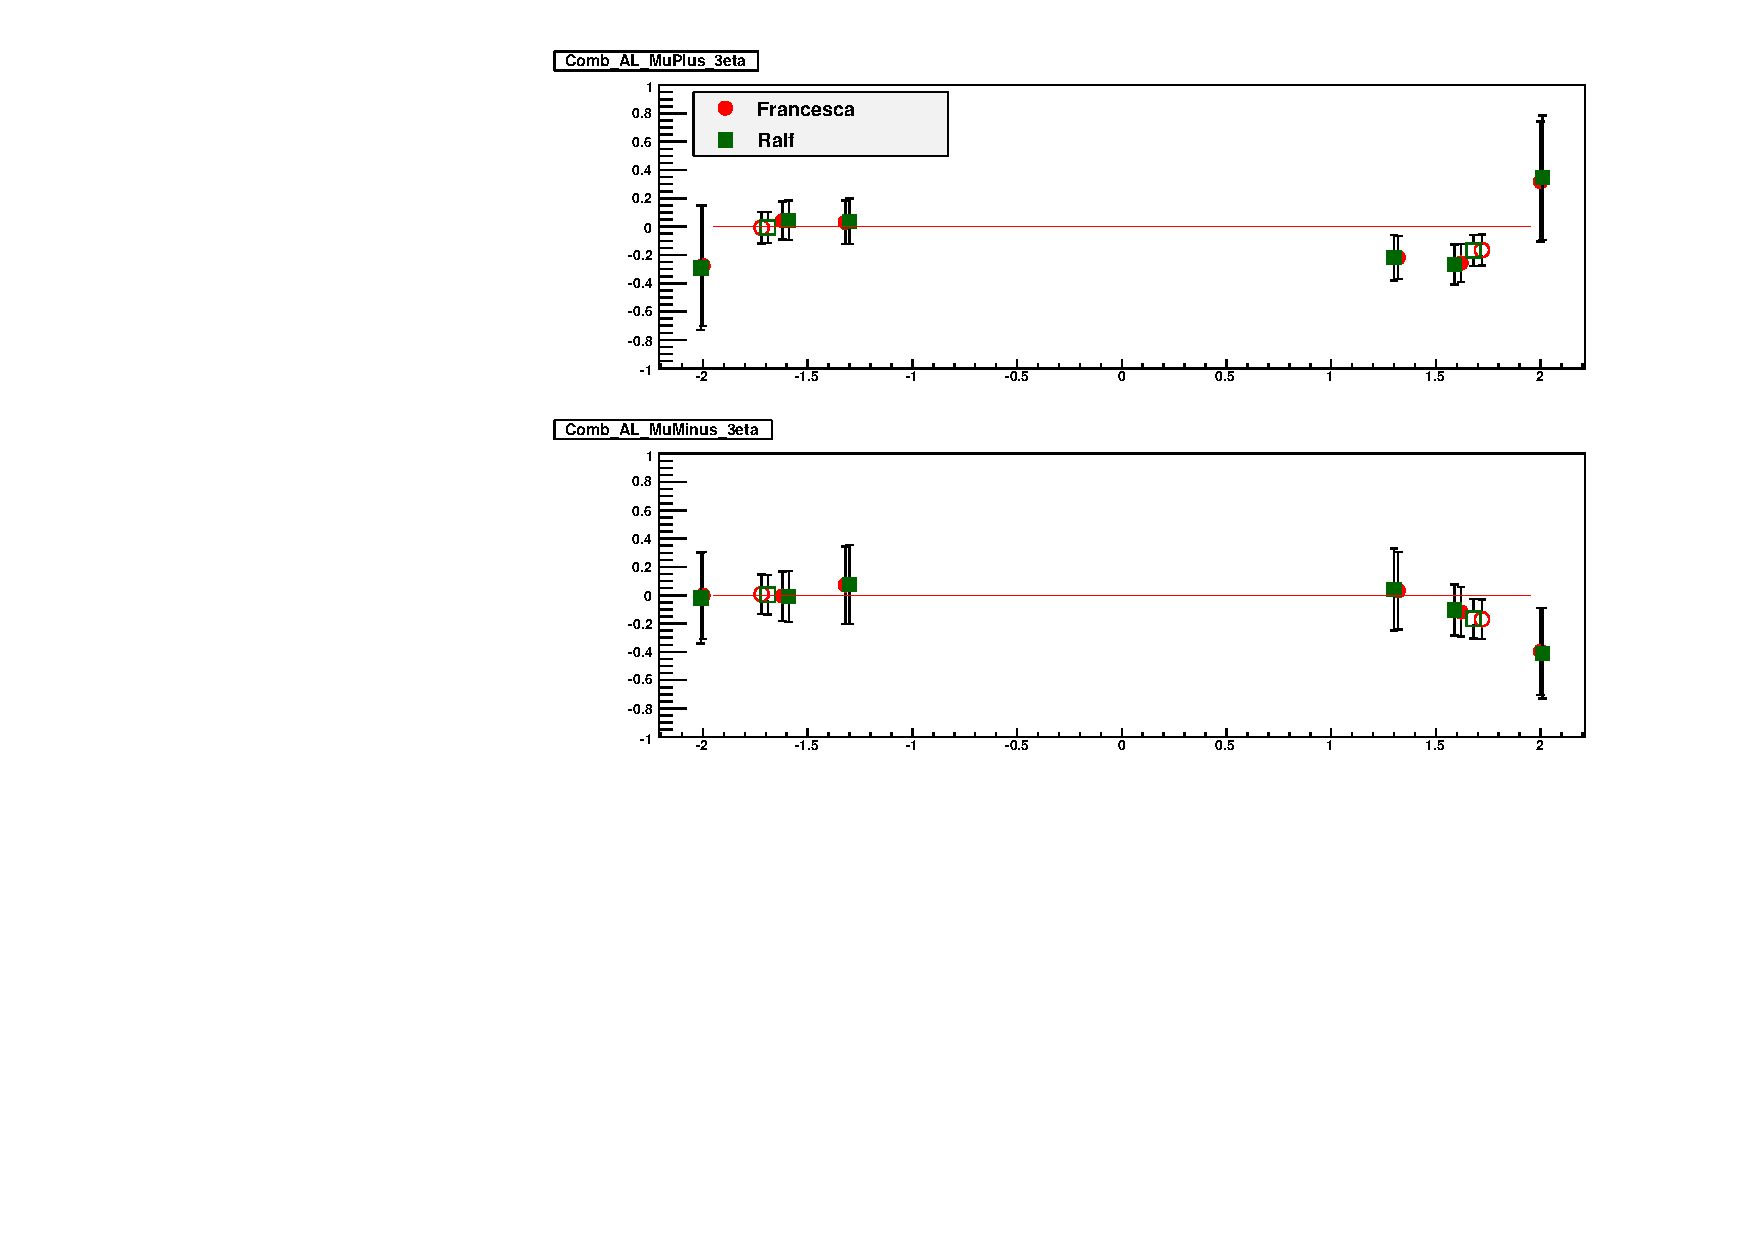
\includegraphics[width=\textwidth]{{../asymmetries/figs/run13/combined_asy_xcheck}.pdf}
\caption{Cross check of the final combined asymmetries between Ralf and Francesca, both using the trees after data selection provided by Ralf.}
\end{center}
\label{fig:asyxc}
\end{figure}

\section{Combined systematic studies}
As could be seen in the previous section, it seems, that using the data-based signal to background extraction in the way introduced in \cite{oide} the resulting background corrected asymmetries are significantly inconsistent with any of the parameterizations. The up and down quark polarizations are generally well enough known, as are the W kinematics, that there is little doubt in the asymmetries mostly related to them, namely the forward $W^-\rightarrow \mu^-$ asymmetries and the backward $W^+\rightarrow\mu^+$ asymmetries. It seems therefore much more likely, that either a statistical fluctuation or analysis error creates the resulting discrepancies. When taking the signl to background values at face value a statistical fluctuation is essentially exluded, however, if there is a significant overestimation of these ratios it could still be possible. 
In order to understand the origins of the data parameterization discrepancy better we are studying the asymmetries and the signal to background ratios as a function of various relevant variables. In most cases the background corrected asymmetries as well as the signal to background ratios are displayed together to give a better idea of the impact on the background. Either the data-based or W-MC based signal to background ratios are displayed and used to see the difference it makes.
\subsection{Asymmetries as function of W selection and deflection angular bands}
As the asymmetry calculation only uses the dw23 region with supposedly W support the whole region and the inverse selection are also of interest. As the inverse region is expected to be dominated by more background its asymmetries should be closer to zero as only the W/Z production gives parity violating asymmetries. However, it seems, that while statistical uncertainties are generally larger the asymmetries have a tendencey to be nonzero in particular also the double spin asymmetries. This could either be an indication of remaining signal in the sidebands or some remaining background asymmetries. The Asymmetries in the dw sidebands can be seen in Figs.~ \ref{fig:dwcuts}
\begin{figure}[ht]
\begin{center}
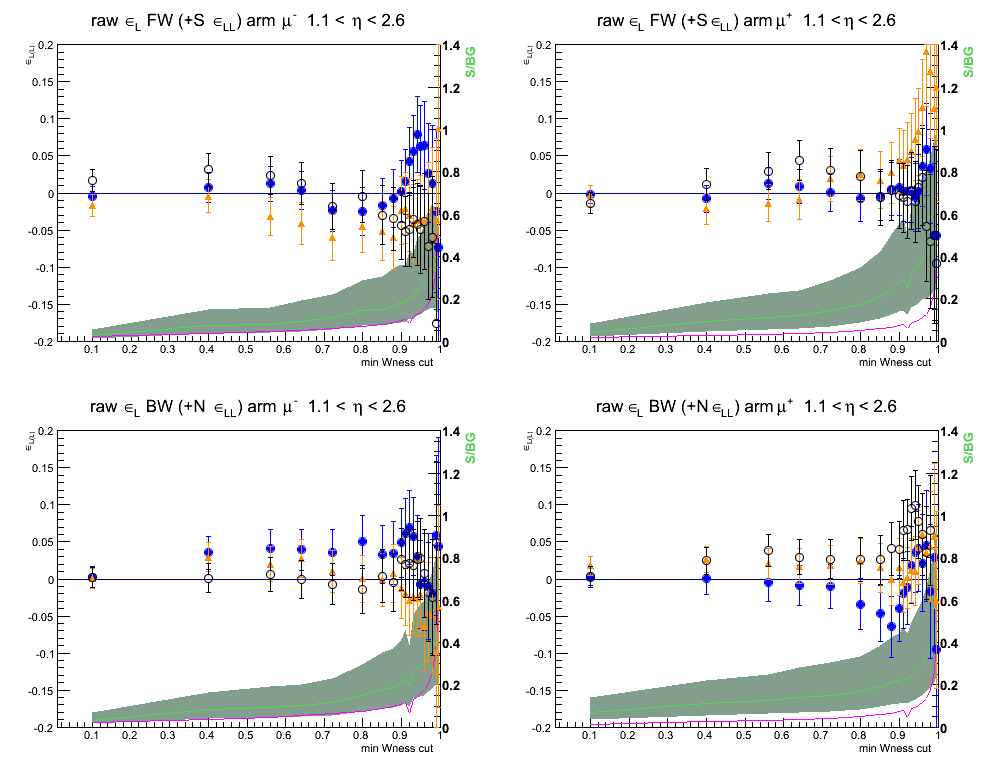
\includegraphics[width=\textwidth]{{../asymmetries/figs/run13/asyvsfcut13_wness_eta3_16_60_dw2}.png}
\caption{Raw asymmetries $\epsilon_{L}$ for the Blue (blue symbols) and Yellow (orange symbols) beams and $\epsilon_{LL}$ (black symbols) for both arms and charges as a function of the preselection range. The combination of all rapidities in one bin after selecting the {\bf sideband} dw23 region is displayed. In addition the extracted signal to background ratios are displayed using the right-hand axis values. The green line displays the data-based extraction method while the magenta line represents the MC signal based extraction.\label{fig:dwcuts}}
\end{center}
\end{figure}

\subsection{Asymmetries and Signal to BG ratio as a function of rate, time and transvsere momentum range}
Another important test is whether the asymmetries show any kind of rate or run dependence effect. For this purpose the data was split up into three rapidity ranges with about equal luminosity: The multi-collision parameters were chosen as 0, 0.69, 0.83, 2. Naively a rate dependent effect would result in a certain ordering of the asymmetries with either increasing or decreasing asymmetries as the rates increase. All the asymmetries as a function of minimum wness cut are displayed in Fig.~ \ref{fig:rateranges}. Out of the 12 different asymmetries ( arm x charge x singe,double spin asymmetry) a few display such a behavior while the majority appears to be randomly distributed between the different rates. 
\begin{figure}[ht] % %does not exists!
\begin{center}
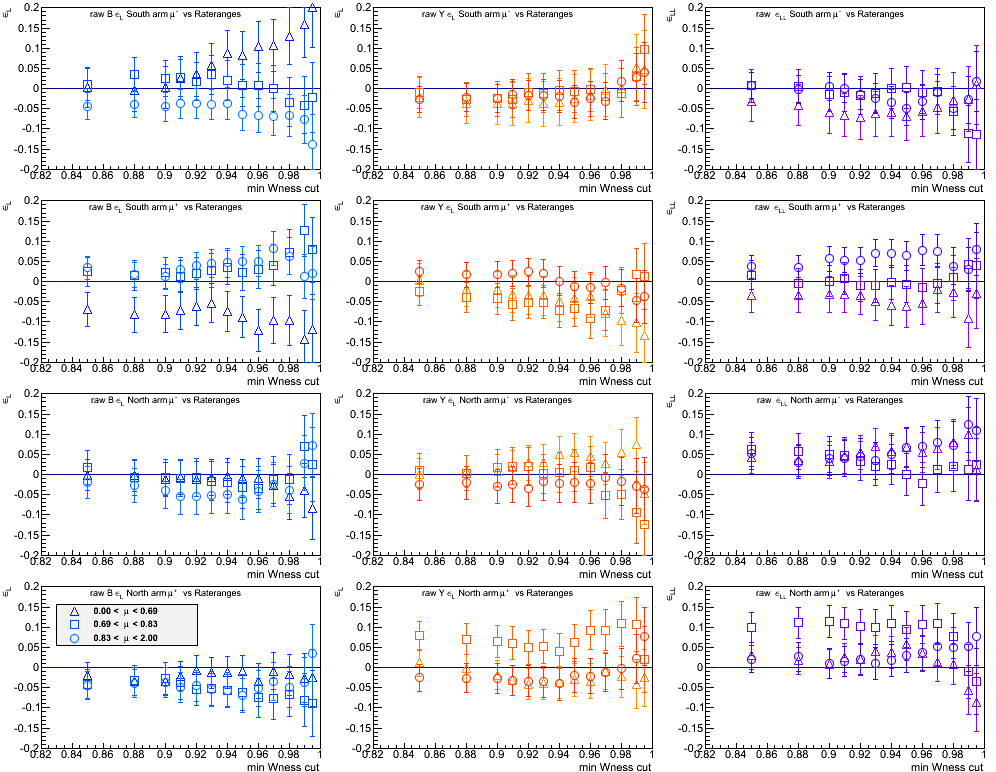
\includegraphics[width=\textwidth]{{../asymmetries/figs/run13/asyvsfcut13_wness_16_60_dw6}.png}
\caption{Raw asymmetries as a function of minimal wness cut when splitting the data sample into three nearly equal luminosity bins of increasing BBC rate in the order of open triangles, open squares and open circles. Each plot displays one asymmetry for each arm and charge. The central dw23 region has been selected.  In addition the extracted signal to background ratios are displayed using the right-hand axis values. The green line displays the data-based extraction method while the magenta line represents the MC signal based extraction.\label{fig:rateranges}}
\end{center}
\end{figure}

A t-test between low and high to intermediate rates was performed and the distribution is given in Fig.~ \ref{fig:raterangest}. The amount of larger differences is on the order expected for statistical fluctuations around an average value and therefore one can conclude, that no obvious rate dependent effect is visible.   
\begin{figure}[ht]
\begin{center}
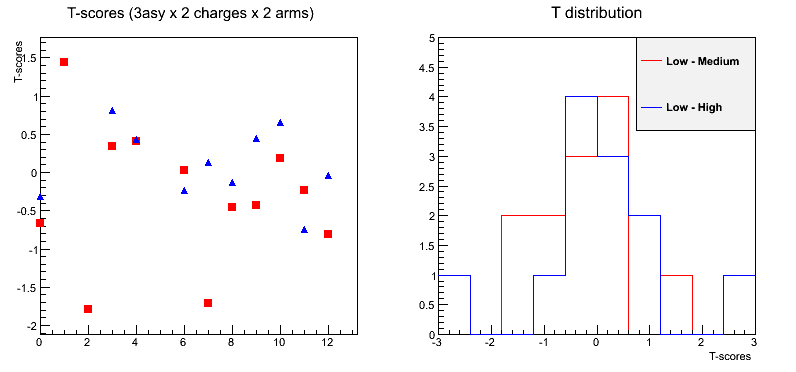
\includegraphics[width=\textwidth]{{../asymmetries/figs/run13/tscores13_wness_16_60_dw6}.png}
\caption{Student T scores and distribution when comparing the lot to medium and the low to high rate subset.\label{fig:raterangest}}
\end{center}
\end{figure}

Similarly, the run dependence was studied in three range bins from 0, 392276, 395770, 399000. While some correlation with the rates is likely, it should be mostly washed out as the collision rates decrease within fills. With the run dependence it would be possible to see, if time dependent detector or accelerator related effects bias the results in some way. 
The resulting asymmetries can be seen in Fig.~ \ref{fig:runranges} and the corresponding t-test between low, high and mid run ranges is given in Fig.~ \ref{rig:runrangest}. Again, while some asymmetries show a range dependence the overall distribution of differences as consistent with fluctuations only.  


\begin{figure}[ht] 
\begin{center}
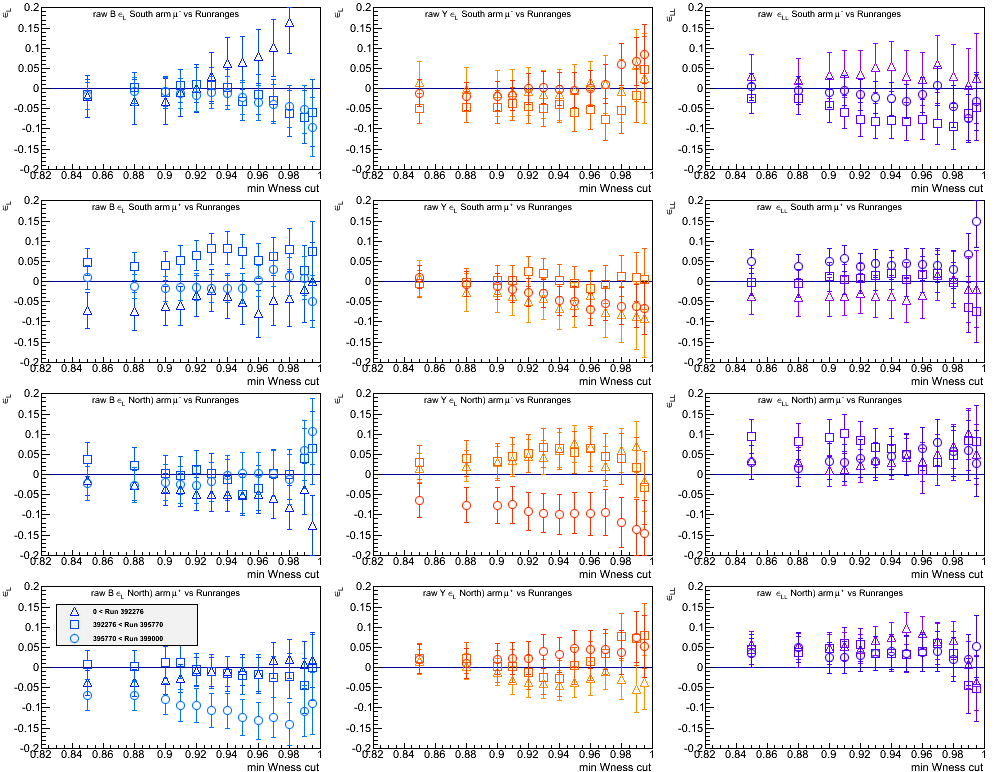
\includegraphics[width=\textwidth]{{../asymmetries/figs/run13/asyvsfcut13_wness_16_60_dw3}.png}
\caption{Raw asymmetries as a function of minimal wness cut when splitting the data sample into three nearly equal luminosity bins of increasing run number in the order of open triangles, open squares and open circles. Each plot displays one asymmetry for each arm and charge. The central dw23 region has been selected.  In addition the extracted signal to background ratios are displayed using the right-hand axis values. The green line displays the data-based extraction method while the magenta line represents the MC signal based extraction.\label{fig:runranges}}
\end{center}
\end{figure}

\begin{figure}[ht]
\begin{center}
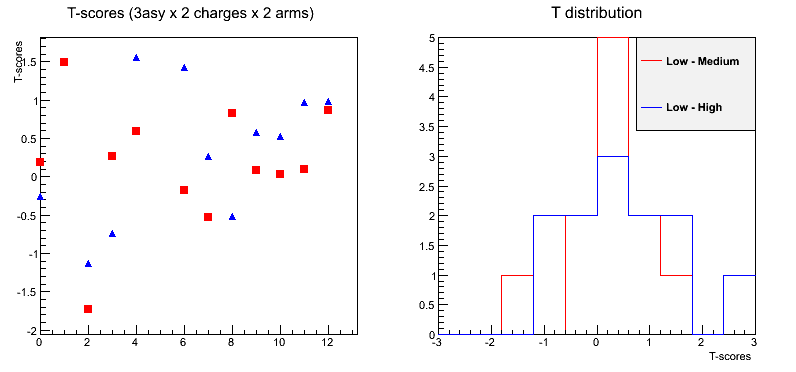
\includegraphics[width=\textwidth]{{../asymmetries/figs/run13/tscores13_wness_16_60_dw3}.png}
\caption{Student T scores and distribution when comparing the lot to medium and the low to high run number subset\label{fig:runrangest}}
\end{center}
\end{figure}


Another test is the dependence on the minimum transverse momentum cut or the transverse momentum range selected. As mentioned earlier in this analysis note the W and Z decay muons dominate at larger transverse momenta while at lower transvsere momenta even more dilution from other muon processes and fake hadrons contribute. As a consequence any asymmetry should be largely diluted and start to appear as the minimum transvsere momentum cut is increased. 
Such a behavior can be seen in Fig.~ \ref{fig:minptasymmetries} where essentially all asymmetries are consistent with zero at low transverse momenta and then increase in some of the cases. What appears different than expectation is the signal to background ratio obtained from the fits. The signal to background ratios from the fits seem to be not increasing while the MC based signal to background ratios show the expected behavior. 
\begin{figure}[ht] 
\begin{center}
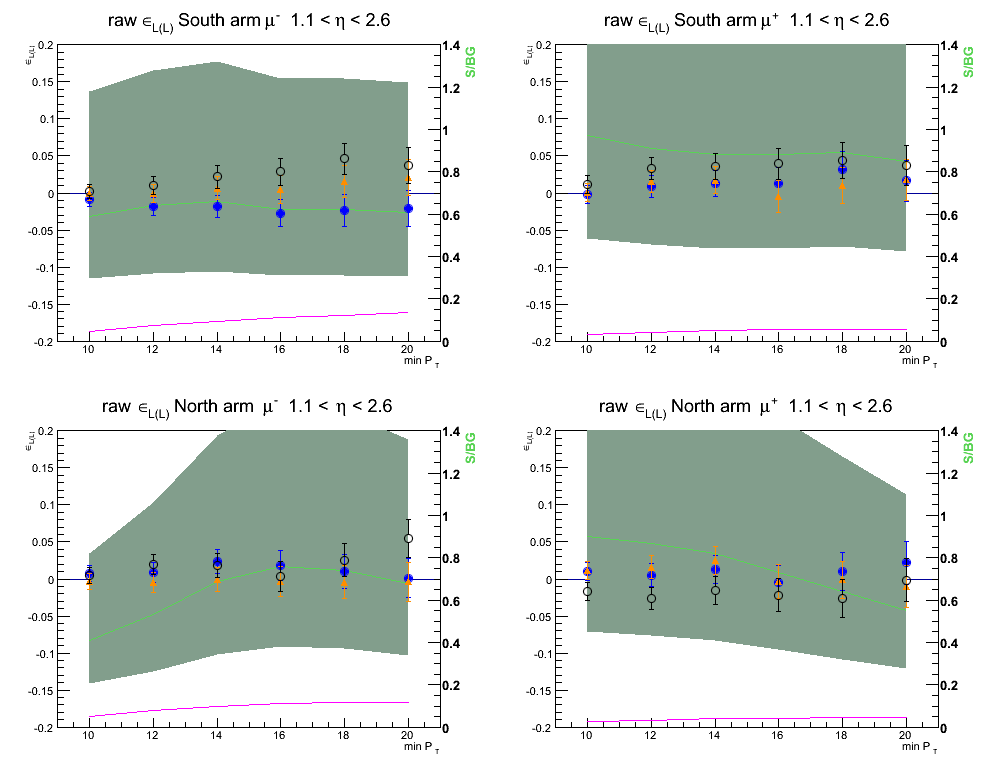
\includegraphics[width=\textwidth]{{../asymmetries/figs/run13/asyvspt13_wness_eta3_0.920_dw0}.png}
\caption{Raw asymmetries $\epsilon_{L}$ for the Blue (blue symbols) and Yellow (orange symbols) beams and $\epsilon_{LL}$ (black symbols) for both arms and charges as a function of the minimal transvsere momentum cut are displayed. In addition the extracted signal to background ratios are displayed using the right-hand axis values. The green line displays the data-based extraction method while the magenta line represents the MC signal based extraction.\label{fig:minptasymmetries}}
\end{center}
\end{figure}

The asymmetries in ranges of transverse momenta are shown in Fig.~ \ref{fig:rangeptasymmetries}. After small initial asymmetries they are mostly consistent at intermediate transvserse momentum ranges and only seem to change again at transverse momenta of around 18. The signal-to-background distribution is again unexpected as obtained from the fits while it is more consistent with expectations in the MC based extraction.  
\begin{figure}[ht]  %does not exists!
\begin{center}
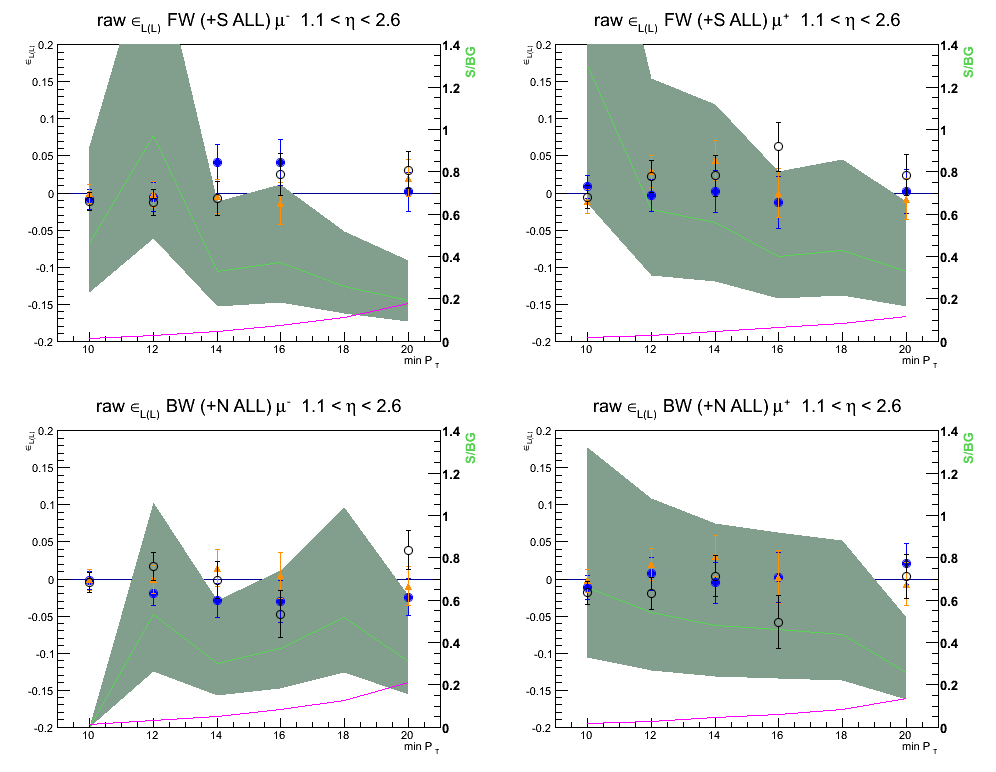
\includegraphics[width=\textwidth]{{../asymmetries/figs/run13/asyvspt13ptslices_wness_eta3_0.920_dw0}.png}
\caption{Raw asymmetries $\epsilon_{L}$ for the Blue (blue symbols) and Yellow (orange symbols) beams and $\epsilon_{LL}$ (black symbols) for both arms and charges as a function of transvsere momentum are displayed. The combination of all rapidities in one bin after selecting the central dw23 region is displayed. In addition the extracted signal to background ratios are displayed using the right-hand axis values. The green line displays the data-based extraction method while the magenta line represents the MC signal based extraction.\label{fig:rangeptasymmetries}}
\end{center}
\end{figure}


 \subsection{Addition of artifical MC-based signal and asymmetries}
Another type of test uses the generated signal MC and includes a fraction of it into the data set before calculating asymmetries and signal to background ratios. In order to do so, crossings are asigned randomly to the MC such, that a certain set of asymmetries can be generated. As an initial test only constant asymmetries were generated. Not any asymmetries can be physically created as the yields in the 4 helicity combinations need to non-negative. The double spin asymmetries need to be within a certain range of the other two.  
The initial asymmetries created were 40\% and 10\% for the negative generated muons and -20\% and -30\% for the positve generated muons while no double spin asymmetries were generated.

\begin{figure}[ht]  %does not exists!
\begin{center}
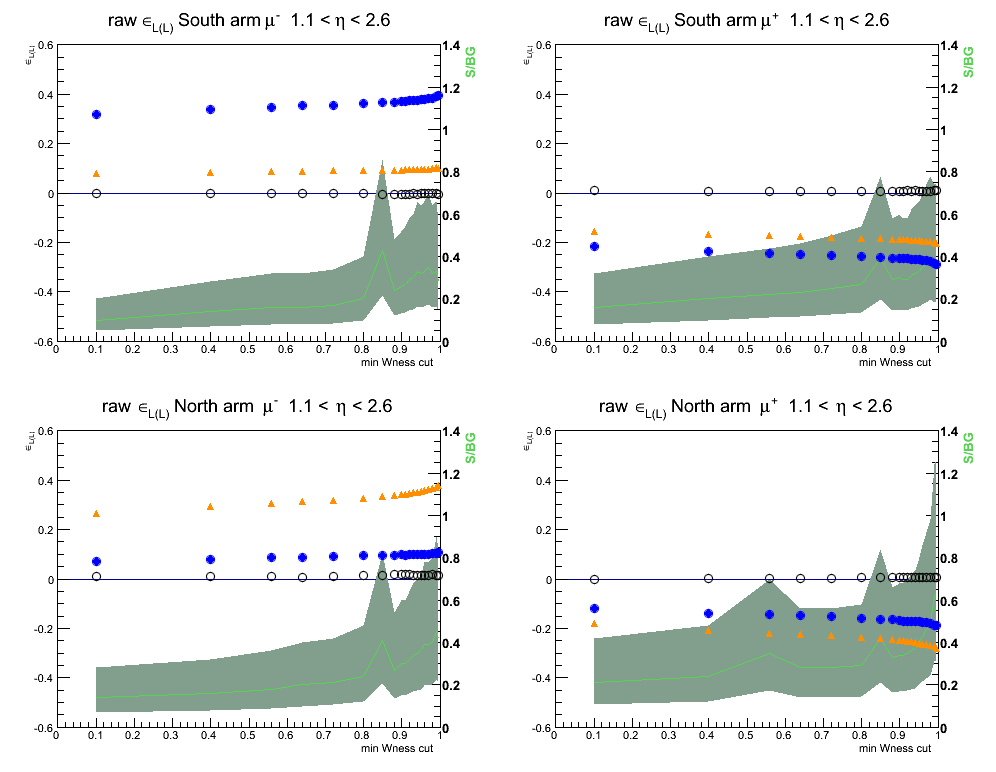
\includegraphics[width=\textwidth]{{../asymmetries/figs/run13/asyvsfcut13_wness_eta3_16_dw1000}.png}
\caption{Raw asymmetries $\epsilon_{L}$ for the Blue (blue symbols) and Yellow (orange symbols) beams and $\epsilon_{LL}$ (black symbols) for both arms and charges as a function of the minimum wness cut are displayed with a fixed signal MC addition of 20 fb$^{-1}$. The combination of all rapidities in one bin after selecting the central dw23 region is displayed. In addition the extracted signal to background ratios are displayed using the right-hand axis values. The green line displays the data-based extraction method while the magenta line represents the MC signal based extraction. \label{fig:mcadd1}}
\end{center}
\end{figure}

The resulting asymmetries and signal-to-background ratios are displayed in Fig.~ \ref{fig:mcadd1} for an MC admixture of 20 fb$^{-1}$ as a function of the minimum wness cut. One can see, that with increasing minimum wness the resulting asymmetries begin to increase as expected while the generally fall short of the generated asymmetries. In Fig.~ \ref{fig:mcadd3} the asymmetries and signal-to-background ratios are displayed as a function of the MC admixture. Also the background corrected asymmetries are displayed which should return the generated asymmetries with the exception of the actual signal based asymmetries in the actual data.   
As one can see, the asymmetries are not properly recovered especially at low admixtures. While part of it could be coming from the Physics asymmetries its contribution should be small. Again, using the MC based signal to background ratios seem to better recover the generated asymmetries.   

\begin{figure}[ht] 
\begin{center}
%\includegraphics[width=\textwidth]{{../asymmetries/figs/run13/asyvsmcaddition_wness_eta3_0.920_dw1000_corr}.png}
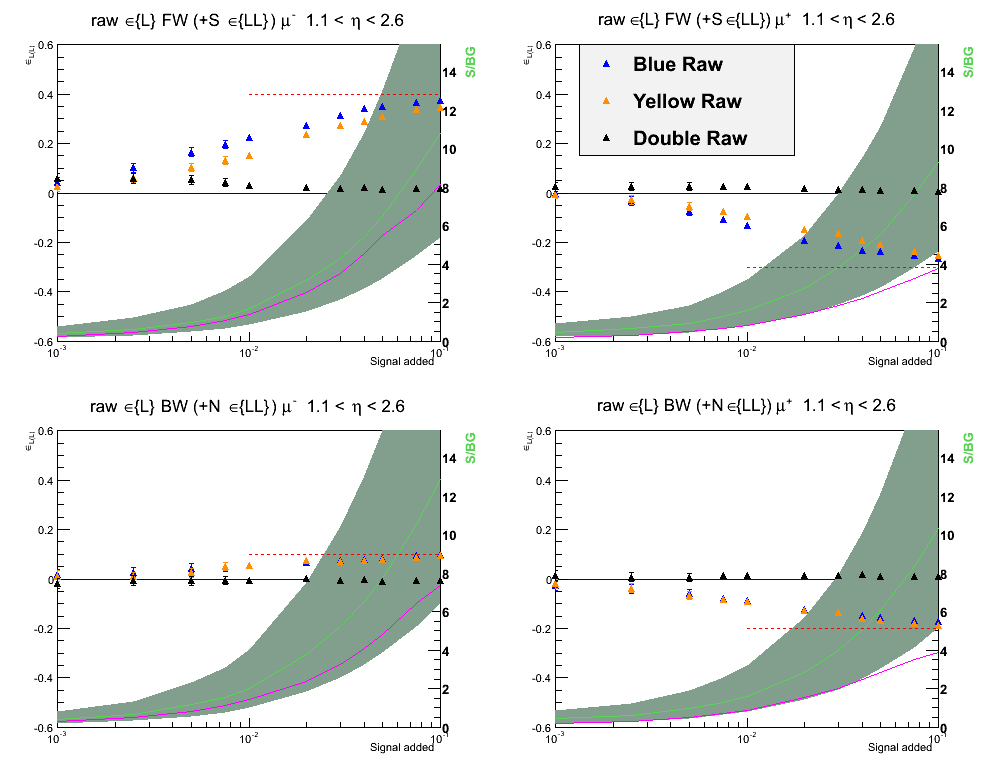
\includegraphics[width=\textwidth]{{../asymmetries/figs/run13/asyvsmcaddition_wness_eta3_0.920_dw1000}.png}
\caption{Raw asymmetries $\epsilon_{L}$ for the Blue (blue symbols) and Yellow (orange symbols) beams and $\epsilon_{LL}$ (black symbols) for both arms and charges as a function of the total Signal MC added are displayed. The combination of all rapidities in one bin after selecting the central dw23 region is displayed. In addition the extracted signal to background ratios are displayed using the right-hand axis values. The green line displays the data-based extraction method while the magenta line represents the MC signal based extraction. The background corrected asymmetries using either the fit based S/BG values (downward open triangles) or old extraction (upward open triangles) are also displayed.\label{fig:mcadd3}}
\end{center}
\end{figure}



 
\subsection{Checking the relative luminosities between patterns}
In the previous evaluation of the asymmetries we were implicitely assuming that we took the same luminosity for every spin pattern.
To make sure this is the case, we explicitely counted the scalers from the spin Data Base from the entry ScalerBbcNoCut for each spin pattern and we found the following:
%\begin{table}
\begin{center}
\begin{tabular}{|c|c|}
Spin Pattern (Blue, Yellow) & \\
\hline 
+1, +1 & 5.29+11\\
-1, +1 & 5.28e+11\\
+1, -1 & 5.29e+11\\
-1, -1 & 5.29e+11.\\
\hline 
%\caption{Scalers count for every spin pattern.}
\end{tabular}
\end{center}
%\end{table}
As can be seen in the previous table, there is only a 0.2\% difference between the luminosity of the spin patterns,
so the previous assumption that there are no differences in luminosities between spin patterns is safe. As a double check,
we rescaled the yield for each spin pattern according to the scalers just reported, and as expected no significant differences
were observed in the combined asymmetries, as shown in figure~\ref{fig:asyscaled}.

\begin{figure}[ht]
\begin{center}
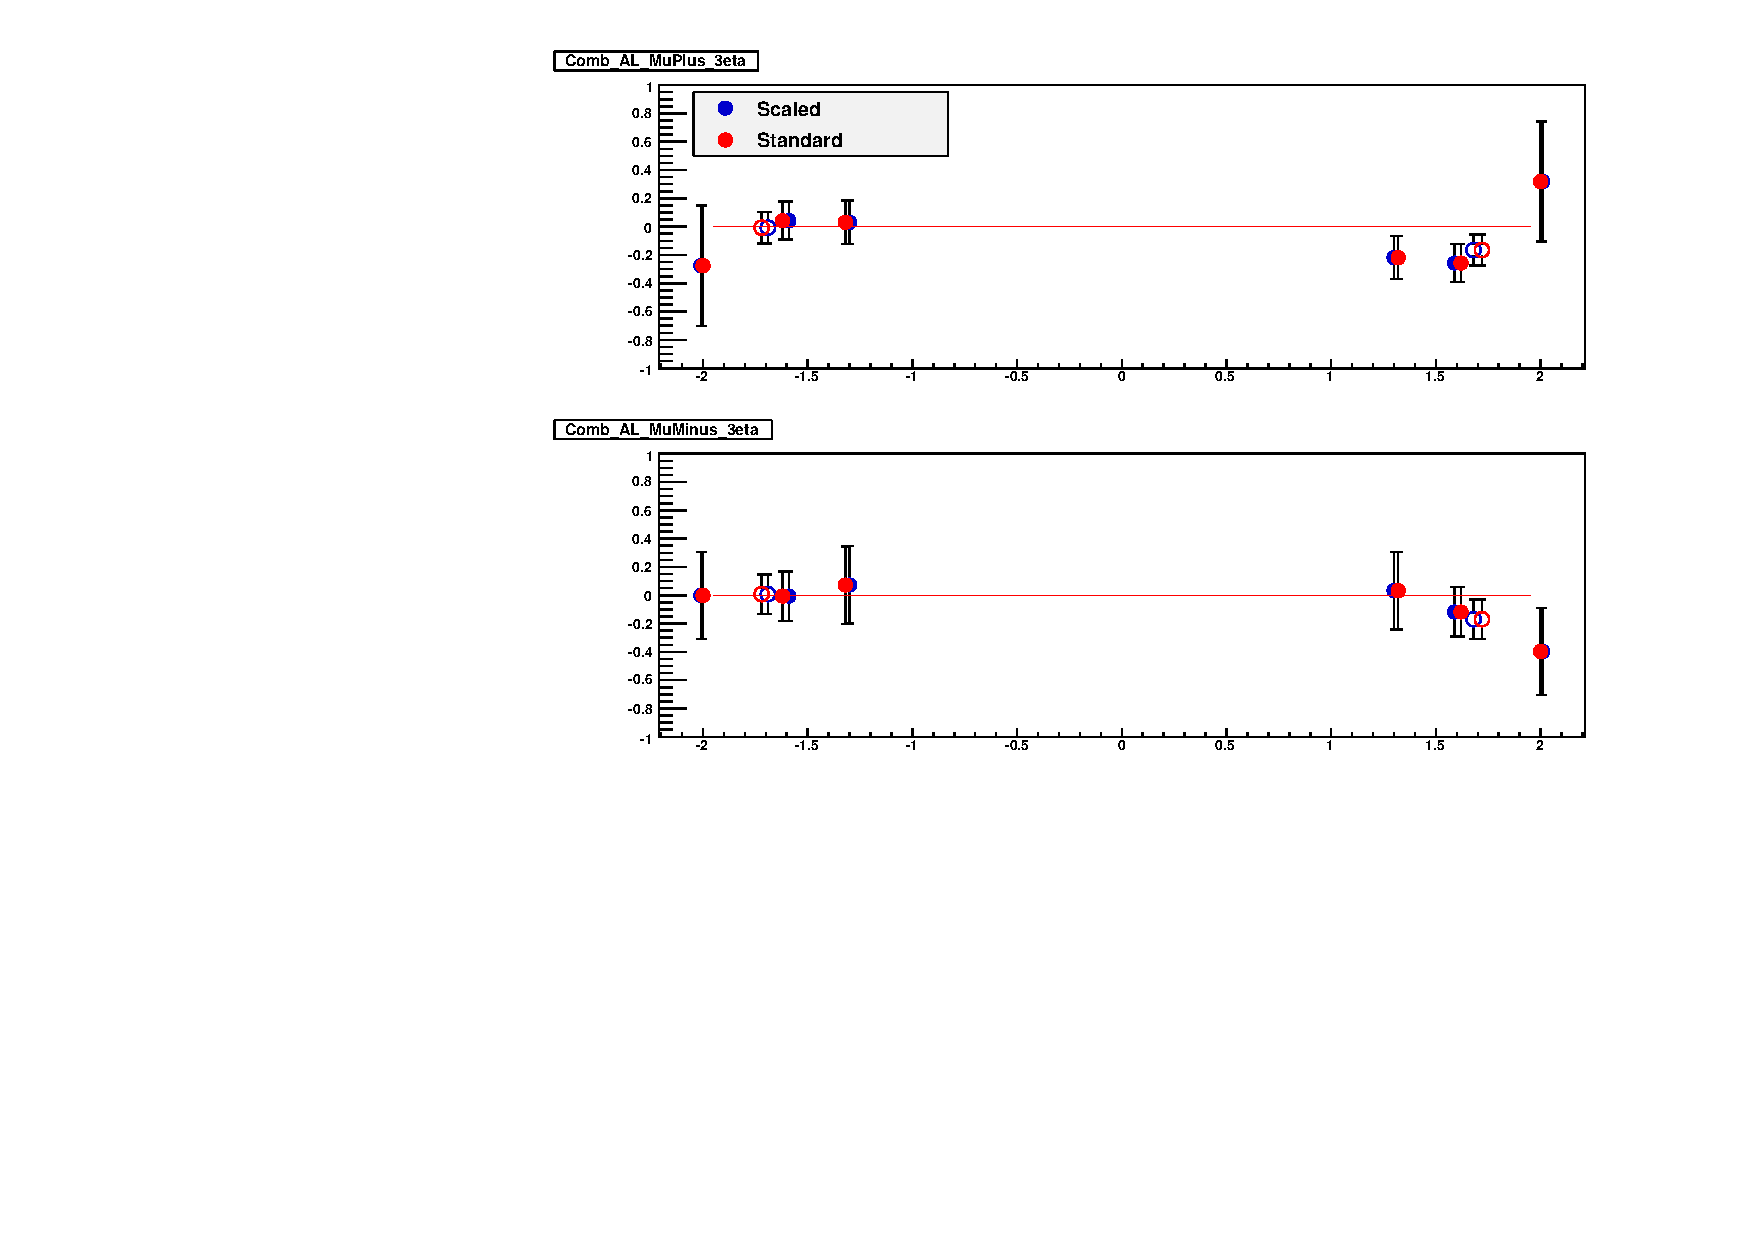
\includegraphics[width=\textwidth]{{../asymmetries/figs/run13/combined_asy_scaled}.pdf}
\caption{Comparison between the combined asymmetries with (in blue) and without (in red) the yield rescaling 
by the relative luminosity of each spin pattern.}
\end{center}
\label{fig:asyscaled}
\end{figure}
